\documentclass[a4paper]{article}
\usepackage{fancyhdr}
\usepackage[usenames, dvipsnames]{xcolor}
\usepackage{graphicx,hyperref,amsmath,float,subfigure,soul}
\usepackage[top=3cm,bottom=3cm,left=3cm,right=3cm]{geometry}
\hypersetup{
	colorlinks,
	citecolor=black,
	filecolor=black,
	linkcolor=black,
	urlcolor=black
}
\newcommand{\HRule}{\rule{\linewidth}{0.5mm}}
\pagestyle{fancy}
\lfoot{\small \color{gray}Tom Peerdeman - 10266186}
\cfoot{\thepage}
\rfoot{\small \color{gray}Ren\'e Aparicio Sa\'ez - 10214054}
\lhead{\small \color{gray} Hadoop}
\begin{document}
	\begin{titlepage}
	\begin{center}
		\textsc{\Large Concurrency \& Parallel Programming}\\[0.5cm]
		\HRule \\[0,4cm]
		\textsc{\huge \bfseries Hadoop}
		\HRule \\[8cm]
		\begin{minipage}{0.4\textwidth}
			\begin{flushleft}\large
				\emph{Auteurs: Tom Peerdeman \& Ren\'e Aparicio Saez}\\
			\end{flushleft}
		\end{minipage}
		\begin{minipage}{0.4\textwidth}
			\begin{flushright}\large
			\emph{Datum: 03-12-2012\\\hspace{1cm}}\\
			\end{flushright}
		\end{minipage}
	\end{center}
	\end{titlepage}

  \section{What is Hadoop}
    Hadoop is a piece of software software that allows certain programs to
    be split in smaller parts in such a way that multiple computations can
    be done on multiple nodes at the same times. In that way the time needed
    to compute the code decreases. It is however necessary that the parts
    have no dependencies of one another.
    
  \subsection{Hadoop's origin}
    Hadoop was created by looking at the MapReduce and Google File System
    papers made by Google. The essence of MapReduce is used by Hadoop.
    The master node takes input. This input is then divided in smaller parts
    and distributed onto worker (or slave) nodes. These worker nodes do all
    the computing. The workers cannot communicate with eachother,
    this is why there must be no dependencies what so ever in the given parts.
    When the workers are done they send their results back to their
    master. The master waits for all the answers and combines all the results
    to form an output.
    
  \subsection{Scalable}
    Hadoop is scalable. This means that the speedup increasement will stay
    roughly the same, despite the amount of work you give to Hadoop.
    For example, a small job can have a speed up of 20\% with Hadoop on four
    worker nodes. A bigger job will also have around 20 \% speedup on four
    worker nodes.
    
  \subsection{Architecture}
    Hadoop uses a special Distributed File System called the Hadoop
    Distributed File System or HDFS. HDFS uses location awareness to tell
    the master where and what each worker is doing. This way, work that must
    be done can be scheduled more efficiently. Also, if an exception is caused
    on a worker, the master will know what happened. If an exception occured
    it resends the job to be computed again.\\
    To know all this, a master node consists of four parts: a JobTracker,
    a TaskTracker, a NameNode and a DataNode. The worker however, only has a
    TaskTracker and a DataNode.
    NameNodes contain information about where data is kept, but does not store
    data itself. Data is kept inside DataNodes. The NameNodes connect to 
    DataNodes to tell them where the data is.
    The JobTracker talks to the NameNode
    to see what data can be sent. If data is found it makes contact with a
    TaskTracker of an open node and sends the information of the NameNode
    to this node. Preferably it sends the task to an empty slot of a node
    on the same server, else the task is send to any empty slot in the same
    rack of machines. If the TaskTracker accepted the node it either tells
    the JobTracker it is completely full or that it still has room for more
    work. These TaskTrackers then start sending messages back, telling the
    JobTracker that everything is ok, or if something went wrong that they
    failed at their job. If the latter happened, JobTracker can send out
    the task to a new node again. When everything happened according to plan,
    the JobTracker changes the status of the worker from occupied to free.
    
  \section{BioHadoop speedup}
    As an example, the speed up is measured for a program that searches,
    arranges and aligns sequences of proteins. This can be done sequential.
    Hadoop can be used to parallelize the program. To measure the speed up,
    multiple tests are run with an increasing amount of worker nodes. The
    Hadoop results can then be compared with the results from the sequential code.
    
  \subsection{Difference between Hadoop and Sequential}
  %TODO explain the difference between Hadoop and sequential
  
  \subsection{Results}
    These are the results gathered from the test runs.
    \begin{table}[H]
	    \label{table:hadoop}
	    \caption{Numerical speedup with increasing splits in Hadoop}
	    \begin{center}
		    \begin{tabular}{| c | c | c | c | c | c |}
			    \hline
			    Sequential & 1 Split & 2 Splits & 4 Splits (+1) & 8 Splits (+1) & 16 Splits (+1)\\ 
			    \hline
			    3m 51.018s & 6m 11.580s & 4m 39.198s & 2m 47.940s & 2m 15.707s & 1m 3.840s\\
			    \hline
			    3m 53.448s & 6m 13.266s & 3m 53.196s & 2m 44.663s & 2m 13.942s & 1m 3.763s\\
			    \hline
			    3m 50.621s & 6m 14.353s & 4m 42.668s & 2m 45.363s & 2m 14.414s & 1m 3.453s\\
			    \hline
			    \multicolumn{6}{|l|}{Average time:}\\
			    \hline
			    3m 51.696s & 6m 13.066s & 4m 25.021s & 2m 45.989s & 2m 14.688s & 1m 3.685s\\
			    \hline
		    \end{tabular}
	    \end{center}
    \end{table}
    \begin{center}
      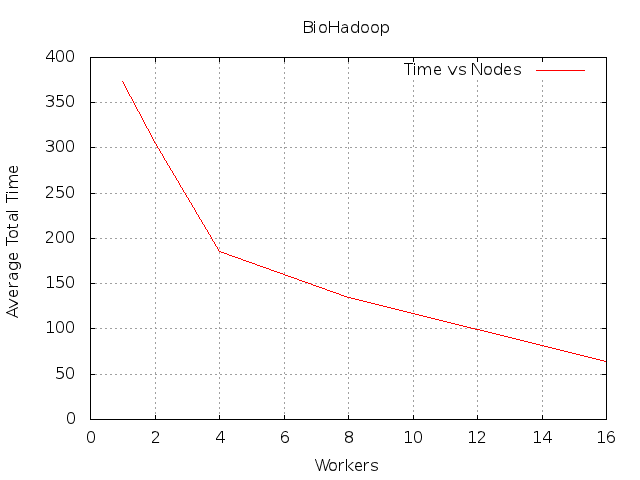
\includegraphics[width=0.7\textwidth]{speedplot.png}
    \end{center}
    In these test runs there where 47550 records to split in total.
    If Hadoop splits these records, it will only assign whole records.
    Alls records that are not assigned are given to an extra node. This is why some of the values in the table
    have a (+1) behind the number of splits.
    The sequential test was run on node069.fs0.das3.cs.vu.nl.\\
    The speedup is shown in the graph below, with one being the
    speed for the sequential code to compute.
    \begin{center}
      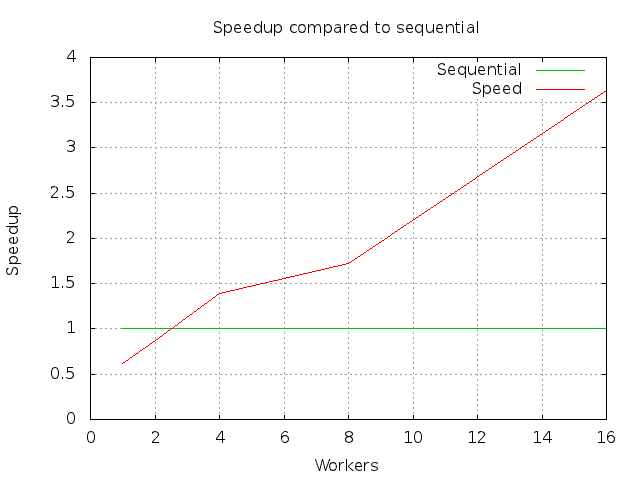
\includegraphics[width=0.7\textwidth]{speedup.png}
    \end{center}
  \subsection{Discussion}
    Hadoop is faster then the sequential code if it has 4 or more workers
    available with this program. This has to do with the communication
    between the TaskTracker(s). When there are only a few nodes,
    this takes more time to setup then the sequential code needs to compute.
    Hadoop also reads the inputfiles twice. The first time to see how many
    each split will get and the second time to really read the file for the program.
    The time needed to compute the program seems to be decreasing exponentially
    when more workers are added. This seems logical, due to the fact that
    parallalization only works onto a certain point when it comes to faster
    computations.
  \subsection{Optimization}
    %TODO how to optimize the code
  
\end{document}
